\documentclass[11pt,a4paper]{article}
\usepackage[left=20mm,right=15mm,top=15mm,bottom=15mm]{geometry}
\usepackage[utf8x]{inputenc}
\usepackage[L7x]{fontenc}
\usepackage[lithuanian]{babel}
\usepackage{tikz}
\usepackage{pgfplots}
\pgfplotsset{compat=newest}
\begin{document}
\begin{titlepage}
  
  \begin{center}
    \textsc{\LARGE Vilniaus Gedimino Technikos universitetas}\\[2mm]
    \textsc{\Large Elektroninių sistemų katedra}\\[70mm]
    \textsc{\Large Terminės difuzijos proceso tyrimas, tranzistorių ekvivalentinių grandinių schemų sudarymas ir akustoelektroninio įtaiso projektavimas}\\[10mm]
    \textsc{\normalsize Elektronikos įtaisų kursinio darbo užduotis}\\[40mm]
    \begin{minipage}{1\textwidth}
      \begin{flushright}
        \emph{Darbą atliko:} EI-08/2 gr. studentas\\ Maksim Norkin\\
        \emph{Darbą tikrino:} V.Malinauskas\\
      \end{flushright}
    \end{minipage}
    \vfill
    {\large Vilnius \\ \the\year}
  \end{center}
\end{titlepage}
\tableofcontents
\newpage
\section{Įvadas}
\section{Šiluminė priemaišų difuzija}
Difuzija ( log. \emph{diffusio} - sklidimas ) yra kryptingas medžiagos dalelių skverbimasis jų tankio mažėjimo 
link dėl šių dalelių chaotiško judėjimo. Gaminant puslaidininkinius įtaisus ir puslaidininkinius integrinius grandynus, 
difuzijos reiškinys panaudojamas puslaidininkiams legiruoti. Aukštoje temperatūroje difuzijos būdu į 
paviršinį puslaidininkio sluoksnį įterpus priemaišų, galima pakeisti šio sluoksnio laidumo tipą arba sudaryti lokaliąsias kitokio laidumo stiris.
\subsection{Priemaišų difuzijos mechanizmas ir greitis}
Šiluminė priemaišų difuzija vyksta dėl difunduojančios medžiagos - difuzanto - koncentracijos gradiento.\\
Priemaišiniai atomai į kietuosius kūnus gali skverbtis keliais būdais: užimdami vakansijas, prasiskverbdami tarp mazgų ir pasikeisdami vietomis su gretimais atomais.\\
Tikimiausias yra pirmasis priemaišų atomų difuzijos mechanizmas, nes aukštoje temperatūroje vakansijų gali būti gana daug. 
Jos atsiranda kaip Šotkio arba Frenkelio defektai. Kylant temperatūrai, vakansijų tankis auga, priemaišinių atomų skverbimosi per 
vakansijas tikimybė didėja. Beje, didėjant prasiskverbusių į padėklą priemaišų tankiui ir dėl to mažėjant vakansijų tankiui, svarbesnis 
tampa antrasis priemaišų skverbimosi kelias - per tarpmazgius. Mažiausiai tikėtinas trečiasis priemaišinių atomų skverbimosi būdas, nes 
gretimi atomai gardelės mazguose gali pasikeisti vietomis tik įgiję gana daug energijos.\\
Difuzijos proceso greitį apibūdina difuzijos koeficientas. Šiluminės priemaišų difuzijos koeficientas $D$ paprastai išreiškiamas 
kvadratiniais centimetrais per sekundę ($cm^2/s$). Jo skaitinę vertę reiškia skaičių dalelių, pereinančių per $1\;cm^2$ plotą 
per $1\;s$, kai priemaišos atomų tankio gradientas lygus $1\;cm^{-4}$.\\
Difuzijos koeficientas labai priklauso nuo temperatūros. Jai kylant, difuzijos koeficientas sparčiai didėja. 
Priklausomybė $D(T)$ išreiškiama Arenijaus ($Arrhenius$) lygtimi:\\
\[D = D_0 e^{-W_a/kT};\]
čia $D_0$ - proporcingumo koeficientas; $W_a$ - difuzijos proceso aktyvacijos energija; $k$ - Bolcmano konstanta; $T$ - difuzijos proceso temperatūra.\\
Koeficientas $D_0$ priklauso nuo puslaidininkio ir priemaišos tipo, kristalo-grafinės krypties, 
kuri vyksta difuzija, ir pradinio priemaišų tankio. Aktyvacijos energija $W_a$ priklauso nuo puslaidininkio, 
priemaišos tipo ir difuzijos mechanizmo. Jei į silicį difunduoja boras, tai $W_a \approx 3,7$ eV, jei fosforas, - 4,4 eV.\\
Kadangi koeficientas $D_0$ ir aktyvacijos energijos energija $W_a$ priklauso nuo daugelio veiksnių, 
tai ankstesnė lygtis gerai tinka tik difuzijos koeficiento $D$ priklausomybių nuo $T$ ir $W_a$ pobūdžiui išreikšti. 
Praktikoje priemaišos difuzijos koeficientas randamas iš literatūroje pateikiamų grafikų, sudarytų remiantis eksperimentų rezultatais.
\subsection{Difuzijos procesų teorija}
Difuzijos teorija pagrįsta dviem dėsniais, kuriuos 1855 m. suformulavo šveicarų mokslininkas A.Fikas (\emph{Fick}).\\
Taikydami pirmą difuzijos dėsnį priemaišų difuzijai ir laikydami, kad priemaišiniai atomai skverbiasi į kristalą $x$ ašies kryptimi, galime rašyti:
\[ J(x,t) = - D \frac{\delta N(x,t)}{\delta x}\]
čia $J$ - priemaišos atomų srauto tankis, $N$ - priemaišos atomų tankis, $t$ - laikas.\\
Antro Fiko dėsnio matematinę ištaišką galima išvesti remiantis pirmuoju dėsniu.\\
Imkime ploną sluoksnį $\delta x$ tarp dviejų vienetinio ploto plokštumų, statmenų difuzinio srauto krypčiai. 
Sakykime, kad priemaišos tankis sluoksnyje laiko momentu $t$ yra $N(x,t)$. Prabėgus laikui $\delta t$, 
priemaišos tankis tampa $N(x,t+ \delta t)$. Tada priemaišos atomų skaičiaus pokytis nagrinėjamame sluoksnyje per laiką $\delta t$ yra
\[ [ N (x,t+\delta t ) - N(x,t) ] \delta x = \frac{\delta N(x,t)}{\delta t} \delta t \delta x\]
Priemaišos tankis kinta todėl, kad priemaišos atomų srautas $J(x,t)$, tekantis į nagrinėjamąjį sluoksnį per 1 plokštymą, 
skiriasi nuo ištekančio per 2 plokštumą srauto $J(x+\delta x,t)$. Dėl to, kad šie srautai nevienodi, 
priemaišos atomų skaičiaus pokytį sluoksnyje $\delta x$ per elementarųjį laiką $\delta t$ galima išreikšti formule:
\[ [J(x,t) - J(x + \delta x,t ) ] \delta t = - \frac{\delta J(x,t)}{\delta x} \delta x \delta t. \]
Sulyginę ankstesnes dvi formules, gauname:
\[ \frac{\delta N(x,t)}{\delta t} = - \frac{\delta J(x,t)}{\delta t} \]
Įrašę į šią lygtį srauto tankio išraišką, gauname diferencialinę lygtį, kuria išreiškiamas antrasis Fiko dėsnis:
\[ \frac{\delta N(x,t)}{\delta t} = D \frac{\delta^2 N(x,t)}{\delta x^2} \]
Ši lygtis aprašo primaišos kaupimosi greitį. Ja naudojantis galima nagrinėti difuzijos proceso dinamiką.\\
Išsprendus antro Fiko dėsnio lygti, randama priemaišos tankio priklausomybė nuo difuzijos trukmės ir koordinatės, 
taigi galima apskaičiuoti priemaišos pasiskirstymą kristale bet kuriuo laiko momentu. 
Priemaišos tankio priklausomybė nuo koordinatės vadinama koncentracijos profiliu, arba legiravimo profiliu.\\
Praktikoje pasitaikančias priemaišų difuzijos sąlygas gana greitai atitinka du paprasti teoriniai modeliai: difuzija iš nesenkančio šaltinio ir difuzija iš riboto šaltinio.\\
Laikoma, kad difuzijos šaltinis yra nesenkantis, jeigu priemaišos atomų tankis kristalo paviršiuje nekinta - jeigu $N(0,t) = N_0 = const$, 
kai $t \geq 0$. Atsižvelgus į pradinę sąlygą $N(x,t) = 0$, kai $x \geq 0 $ ir $t=0$, bei ribinę sąlygą $N(x,t)=0$, 
kai $x \rightarrow \infty$ ir $t \geq 0$, gaunamas toks antrosios Fiko diferencialinės lygties sprendinys:
\[N(x,t) = N_0\;erfc\frac{x}{2\sqrt{Dt}}\]
čia erfc - papildoma paklaidų funkcija ( \emph{error function complement} ), išreiškiama formule:
% TODO: REIKIA integralo
\[erfc(y) = 1 - \frac{2}{\sqrt{\pi}} \int^y_0 exp(-y^2) \delta y\]
Dydis $\sqrt{Dt}$ vadinamas difuzijos nuotoliu.\\
Pagal $N(x,t)$ išraišką, priemaišos atomų tankio pasiskirstymą lemia difuzijos koeficientas $D$ ( proceso temperatūra T ) ir difuzijos proceso trukmė $t$. Vykstant difuzijai iš nesenkančio šaltinio, didesniame gylyje priemaišos tankis yra mažesnis. Tam tikrame gylyje, kol vyksta difuzija, priemaišos atomų tankis didėja. Jei difuzijos procesas vyktų pakankamai ilgai, priemaišos atomų tankis bet kuriame gylyje taptų toks, kaip paviršiuje.\\
Nuo difuzijos proceso temperatūros ir trukmės priklauso ir legiravimo dozė $Q$ -  skaičius priemaišos atomų, perėjusių per vienetinį padėklo paviršiaus plotą per difuzijos laiką $t$.\\
Žinodami $N(x,t)$, galime rasti difuzijos srauto tankį. Taikydami pirmajį Fiko dėsnį, galime rašyti:
\[ J(0,t) = - D\frac{\delta N(x,t)}{\delta x}|_{x=0}  \]
Į šią formulę įrašę priemaišos pasiskirstymo išraišką, gauname:
\[J(0,t) = D\frac{N_0}{\sqrt{\pi Dt}} e^{-(x/2\sqrt{Dt})^{2}}|_{x=0} = N_0 \sqrt{\frac{D}{\pi}}\]
Suintegravę priemaišos atomų srautą per vienetinio ploto padėklo paviršių, gauname legiravimo dozę:
\[ Q(t) = \int^{t}_{0}J(0,t)\delta t = ... = 2N_0 \sqrt{\frac{Dt}{\pi}} \]
Praktikoje šiluminės priemaišų difuzijos procesą dažniausiai sudaro dvi stadijas. Difuzija iš nesenkančio šaltinio vyksta pirmojoje - \emph{priemaišų įterpimo} stadijoje. Šioje stadijoje į ploną paviršinį kristalo sluoksnį įterpiamas reikiamas priemaišos kiekis. Antrojoje - \emph{priemaišų perskirstymo} stadijoje - aukštesnėje temperatūroje suformuojamas legiravimo profilis.\\
Dažnai antrojoje difuzijos stadijoje atliekamas ir paviršiaus oksidavimas. Todėl antrojoje stadijoje priemaišiniai atomai per padėklo paviršių neprasiskverbia ir legiravimo dozė nekinta. Tada difuzija vyksta iš riboto šaltinio - iš pirmojoje stadijoje legiruoto paviršinio sluoksnio. Šiomis sąlygomis antrosios Fiko diferencialinės lygties sprendinys išreiškiamas formule:
\[ N(x,t') = \frac{Q}{\sqrt{\pi D't'}} exp \left (-\frac{x^2}{4D't'} \right ) \]
čia $D'$ - priemaišos difuzijos koeficientas priemaišų perskirstymo etape, t' - šio etapo trukmė.\\
Pastaroji formulė atitinka Gauso ( Gauss ), arba normalųjį, pasiskirstymą. Kreivių parametras yra difuzijos koeficiento ir proceso trukmės sandauga.


\section{Difuzijos proceso tyrimas}
\subsection{Apskaičiuoti ir nubraižyti priemaišų pasiskirstymą po priemaišų įterpimo etapo}
Pradiniai duomenys:\\
Difuzijos koeficienas ($cm^2/s$): $D = 1.8*10^{-13}$\\
Proceso trukmės: $t_1 = 13min = 780s, t_2 = 18min = 1080s$ ir $t_3 = 22min = 1320s$.\\
Difuzija iš nesenkančio šaltinio vyksta pirmojoje - priemaišų įterpimo stadijoje. Jos pasisskirstymas randamas, pasitelkus:
\[N(x,t) = N_0*erfc \left( \frac{x}{x\sqrt{Dt}} \right) \] \\
\begin{tikzpicture}[domain=0:0.005]
  \begin{axis} [
      xlabel=$x$,
      ylabel=$N(x)/N_0$,
      grid=major]
    \addplot[smooth, mark=*] plot function {erfc(x/(2*sqrt(1.8*10**(-13)*780)))};
    \addlegendentry{$t_1$}
    \addplot[smooth, mark=o] plot function {erfc(x/(2*sqrt(1.8*10**(-13)*1080)))};
    \addlegendentry{$t_2$}
    \addplot[smooth, mark=x] plot function {erfc(x/(2*sqrt(1.8*10**(-13)*1320)))};
    \addlegendentry{$t_3$}
  \end{axis}
\end{tikzpicture}

\subsection{Apskaičiuoti ir nubraižyti, kaip priemaišų įterpimo etape kinta priemaišos srauto tankis ir legiravimo dozė}
Pradiniai duomenys:\\
Priemaišų koncentracija bandinio paviršiuje ($1/cm^2$): $N_0 = 3*10^{20}$\\
Priemaišos srauto tankis išreiškiamas:\\
\[J(0,t) = N_0*\sqrt{\frac{D}{\pi t}}\]
\begin{tikzpicture}[domain=0:1]
  \begin{axis} [
      xlabel=$t$,
      ylabel=$J(0\,t)$,
      grid=major
    ]
    \addplot[smooth] plot function {3*10**(20)*sqrt(1.8*10**(-13)/(3.14*x))};
  \end{axis}
\end{tikzpicture} \\

Legiravimo dozė išreiškiama:\\
\[Q(t) = 2*N_0*\sqrt{\frac{Dt}{\pi}}\]
\begin{tikzpicture}[domain=0:1]
  \begin{axis} [
      xlabel=$t$,
      ylabel=$Q(t)$,
      grid=major
    ]
    \addplot[smooth] plot function {3*10**(20)*sqrt((1.8*10**(-13)*x)/(3.14))};
  \end{axis}
\end{tikzpicture} \\
\subsection{Apskaičiuoti ir nubraižyti priemaišų pasiskirstymą po priemaišų perskirstymo etapo}
Pradiniai duomenys:\\
Legiravimo dozė ($1/cm^3$): $Q = 1.4*10^{13}$;\\
Difuzijos koeficientas ($cm^2/S$): $D = 1.8*10^{-13}$;\\
Proceso trukmės: $t_1 = 81min = 4860s$; $t_2 = 70min = 4200s$; $t_3 = 21min = 1260s$;\\
Priemaišų perskirstymo stadiją galime apibrėžti:\\
\[N(x,t') = \frac{Q}{\sqrt{\pi D' t'}} exp \left( - \frac{x^2}{4D't'} \right)  \]

\begin{tikzpicture}[domain=0:0.005]
  \begin{axis} [
      ylabel=$N(x)$,
      xlabel=$x$,
      grid=major
    ]
    % Q/sqrt(pi*D'*t')*exp(-(x^2)/(4*D't'))
    \addplot[smooth,mark=*] plot function{ (1.4*10**(13)/(sqrt(pi*1.8*10**(-13)))*exp(-(x**2)/(4*1.8*10**(-13)*4860))) };
    \addlegendentry{$t_1$}
    \addplot[smooth,mark=o] plot function{ (1.4*10**(13)/(sqrt(pi*1.8*10**(-13)))*exp(-(x**2)/(4*1.8*10**(-13)*4200))) };
    \addlegendentry{$t_2$}
    \addplot[smooth,mark=x] plot function{ (1.4*10**(13)/(sqrt(pi*1.8*10**(-13)))*exp(-(x**2)/(4*1.8*10**(-13)*1260))) };
    \addlegendentry{$t_3$}
  \end{axis}
\end{tikzpicture}

\subsection{Apskaičiuoti ir nubraižyti priemaišų pasiskirstymą tranzistoriuje, formuojamame dvikartės difuzijos būdu}

\begin{tabular}{|r|c|c|c|}\hline
  & Įterpimo stadija & Perskirstymo stadija & Įterpimo stadija \\ \hline
  Priemaišų koncentracija ($1/cm^3$): & $2.5*10^{19}$   & -              & $1.4*10^{21}$ \\ \hline
  Normali temperatūra ($^{\circ}C$):   & $1000$         & $1000$         & $1000$ \\ \hline
  Aktyvacijos energija ($eV$):        & $2.2$          & $3.7$          & $2.9$ \\ \hline
  Difuzijos koeficientas ($cm^2/s$):  & $1.9*10^{-13}$  & $1.4*10^{-13}$  & $3.8*10^{-13}$ \\  \hline
  Stadijos trukmė ($min.$):           & $24$           & $77$           & $42$ \\ \hline
  Faktinė temperatūra ($^{\circ}C$):   & $942$          & $1056$         & $318$ \\ \hline
\end{tabular}\\\\\\
% Dvikartė difuzija
% Bazes difuzija
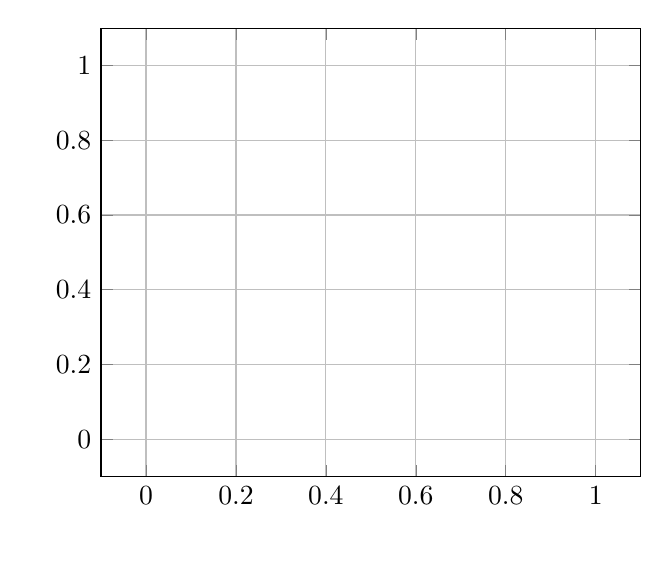
\begin{tikzpicture}[domain=0:0.005]
  \begin{axis} [
      ylabel=$$,
      xlabel=$$,
      grid=major
    ]
    % Q = N_0 * sqrt{ \pi D' t' }
    %                                              Q
    %\addplot[smooth] plot function{ ( 2.5*10^(19)*sqrt(pi*1.9*10^(-13)*24*60) ) };
  \end{axis}
\end{tikzpicture}


\section{Dvipolio tranzistoriaus parametrų skaičiavimas ir ekvivalentinės grandinės schemos sudarymas}
Pradiniai duomenys:\\
$I_B = 0.14 mA = 0.14 * 10^{-3}$, $U_{CE} = 8V$, $f_{T} = 0.9 GHz = 0.9*10^{9}Hz$;\\
\subsection{Rasti dvipolio tranzistoriaus $h$ parametrus}
\subsection{Sudaryti tranzistoriaus $\Pi$ pavidalo ekvivalentinės grandinės schemą, rasti jos elementų parametrus}
\subsection{Apskaičiuoti išėjimo srovės kintamąją dedamąją, kai kintamoji įėjimo įtampa yra 115mV}
\subsection{Rasti žemo dažnio įtampos stiprinimo koeficiantą, kai apkrovos varža lygi 892 $\Omega$ }

\section{Lauko tranzistoriaus parametrų skaičiavimas ir ekvivalentinės grandinės schemos sudarymas}
\subsection{Nubraižyti lauko tranzistoriaus perdavimo charkteristikas, kai $U_{DS} = 3,7,11 V$}
\subsection{Apskaičiuoti lauko tranzistoriaus parametrus nurodytame darbo taške}
\subsection{Sudaryti lauko tranzistoriaus ekvivalentinės grandinės schemą}
\subsection{Apskaičiuoti $f_{T}$, kai $C_{11}$ = 4, $C_{12} = 9$ pF}
\subsection{Apskaičiuoti kintamąją išėjimo srovės dedamąją, kai kintamosios įėjimo įtampos amplitudė yra 135 mV}
\subsection{Rasti žemo dažnio įtampos stiprinimo koeficientą, kai apkrovos varža lygi 621 $\Omega$}

\section{Akustinės elektronikos įtaiso projektavimas}
Pradiniai duomenys:\\
Centrinis pralaidumo juostos dažnis (MHz): 100\\
Pralaidumo juostos plotis (MHz): 8

\end{document}
